% Filename: try21.tex
% This code is part of 'Cursos CAMECC: Introducao ao LaTeX para o Curso 29 - Licenciatura em Matematica'
% 
% Description: This file correspond exercise 21 of the textbook using in the course.
% 
% Created: 07.06.12 11:30:10 AM
% Last Change: 07.06.12 11:30:30 AM
% 
% Authors:
% - Raniere Silva, r.gaia.cs@gmail.com
% 
% Organization: CAMECC - Centro Academico dos Estudantes do IMECC
% 
% Copyright (c) 2012, Raniere Silva. All rights reserved.
% 
% This work is licensed under the Creative Commons Attribution-ShareAlike 3.0 Unported License. To view a copy of this license, visit http://creativecommons.org/licenses/by-sa/3.0/ or send a letter to Creative Commons, 444 Castro Street, Suite 900, Mountain View, California, 94041, USA.
%
% This work is distributed in the hope that it will be useful, but WITHOUT ANY WARRANTY; without even the implied warranty of MERCHANTABILITY or FITNESS FOR A PARTICULAR PURPOSE.
%
\documentclass[12pt, a4paper, twocolumn]{article}
\usepackage[T1]{fontenc} 
\usepackage[utf8]{inputenc}
\usepackage[top=3cm,left=2cm,right=2cm,bottom=3cm]{geometry}
\usepackage[brazil]{babel}
\usepackage{graphicx}
\usepackage{url}

\begin{document}
\nocite{Rodrigues:2009:Ovino}
O FarmPoint fez uma análise dos dados apresentados pelo Instituto Brasileiro de Geografia e Estatística (IBGE) na última quarta-feira, dia 24, sobre a Pesquisa de Produção da Pecuária Municipal de 2009 (PPM 2009). O efetivo de ovinos em 2009 foi de 16,8 milhões de cabeças, crescimento de 1,1\% frente as 16,6 milhões de cabeças de 2008 e o efetivo de caprinos foi de 9,16 milhões de cabeças, queda de 2,04\% comparado as 9,35 milhões de cabeças de 2008. 

\section{Ovinos}

O efetivo de ovinos em 2009 foi de 16,8 milhões de cabeças, crescimento de 1,1\% frente as 16,6 milhões de cabeças de 2008. Em 2009, a região Nordeste deteve o maior número de cabeças ovinas, totalizando 9,56 milhões de cabeças, crescimento de 2,08\% frente a 2008. A região Sul apresentou o segundo maior rebanho, 4,8 milhões de cabeças, queda de 0,81\% comparado a 2008. A região Centro-Oeste apresentou o terceiro maior rebanho, 1,12 milhões de cabeças, crescimento de 1,56\% frente a 2008, seguido da região Sudeste com 761.952 cabeças (queda de 0,39\% frente a 2008) e da região região Norte, 547.903 cabeças, aumento de 2,51\%.

\section{Regiões}
A região Nordeste possui 56,9\% do rebanho nacional, seguida da região Sul (28,6\%), região Centro-Oeste (6,71\%), região Sudeste (4,53\%) e região Norte (3,26\%).

\begin{figure}[htb]
\centering
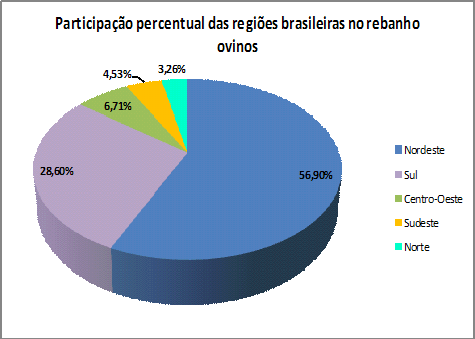
\includegraphics[width=.3\textwidth]{ovinos.png}
\caption{Ovinos}
\label{fig:ovinos}
\end{figure}

\section{Estados}
Em 2009, o Rio Grande do Sul se manteve na liderança e totalizou 3,94 milhões de cabeças, queda de 1,59\% frente a 2008. A Bahia manteve o segundo lugar no ranking, com um efetivo de 3,02 milhões de cabeças e crescimento de 0,25\% frente a 2008. A terceira posição foi ocupada pelo Ceará, com 2,07 milhões de cabeças, crescimento de 1,98\% comparado ao ano anterior. Pernambuco apresentou um crescimento de 10\%, totalizando 1,48 milhões de cabeças e ocupando o quarto lugar. 
\begin{figure}[htb]
\centering
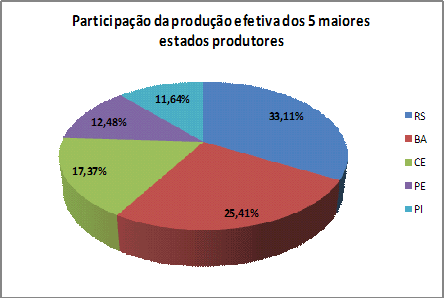
\includegraphics[width=.3\textwidth]{estados.png}
\caption{Estados}
\label{fig:estados}
\end{figure}

\begin{table}[htb]
\centering
\caption{Os 5 municípios com maior rebanho de ovinos em 2009}
\label{tab:mun}
\begin{tabular}{|c|c|}
\hline 
\textbf{Municípios} & \textbf{\# cabeças} \\ \hline
Sant'Ana do Livramento - RS & 401779 \\ \hline
Alegrete - RS & 239778 \\ \hline
Casa Nova - BA & 225832 \\ \hline
Quaraí - RS & 190744 \\ \hline
Uruguaiana - RS & 180407 \\ \hline
\end{tabular}
\end{table}

\bibliography{try21}
\bibliographystyle{plain}
\end{document}
